% Options for packages loaded elsewhere
\PassOptionsToPackage{unicode}{hyperref}
\PassOptionsToPackage{hyphens}{url}
%
\documentclass[
]{article}
\usepackage{amsmath,amssymb}
\usepackage{lmodern}
\usepackage{iftex}
\ifPDFTeX
  \usepackage[T1]{fontenc}
  \usepackage[utf8]{inputenc}
  \usepackage{textcomp} % provide euro and other symbols
\else % if luatex or xetex
  \usepackage{unicode-math}
  \defaultfontfeatures{Scale=MatchLowercase}
  \defaultfontfeatures[\rmfamily]{Ligatures=TeX,Scale=1}
\fi
% Use upquote if available, for straight quotes in verbatim environments
\IfFileExists{upquote.sty}{\usepackage{upquote}}{}
\IfFileExists{microtype.sty}{% use microtype if available
  \usepackage[]{microtype}
  \UseMicrotypeSet[protrusion]{basicmath} % disable protrusion for tt fonts
}{}
\makeatletter
\@ifundefined{KOMAClassName}{% if non-KOMA class
  \IfFileExists{parskip.sty}{%
    \usepackage{parskip}
  }{% else
    \setlength{\parindent}{0pt}
    \setlength{\parskip}{6pt plus 2pt minus 1pt}}
}{% if KOMA class
  \KOMAoptions{parskip=half}}
\makeatother
\usepackage{xcolor}
\usepackage[margin=1in]{geometry}
\usepackage{color}
\usepackage{fancyvrb}
\newcommand{\VerbBar}{|}
\newcommand{\VERB}{\Verb[commandchars=\\\{\}]}
\DefineVerbatimEnvironment{Highlighting}{Verbatim}{commandchars=\\\{\}}
% Add ',fontsize=\small' for more characters per line
\usepackage{framed}
\definecolor{shadecolor}{RGB}{248,248,248}
\newenvironment{Shaded}{\begin{snugshade}}{\end{snugshade}}
\newcommand{\AlertTok}[1]{\textcolor[rgb]{0.94,0.16,0.16}{#1}}
\newcommand{\AnnotationTok}[1]{\textcolor[rgb]{0.56,0.35,0.01}{\textbf{\textit{#1}}}}
\newcommand{\AttributeTok}[1]{\textcolor[rgb]{0.77,0.63,0.00}{#1}}
\newcommand{\BaseNTok}[1]{\textcolor[rgb]{0.00,0.00,0.81}{#1}}
\newcommand{\BuiltInTok}[1]{#1}
\newcommand{\CharTok}[1]{\textcolor[rgb]{0.31,0.60,0.02}{#1}}
\newcommand{\CommentTok}[1]{\textcolor[rgb]{0.56,0.35,0.01}{\textit{#1}}}
\newcommand{\CommentVarTok}[1]{\textcolor[rgb]{0.56,0.35,0.01}{\textbf{\textit{#1}}}}
\newcommand{\ConstantTok}[1]{\textcolor[rgb]{0.00,0.00,0.00}{#1}}
\newcommand{\ControlFlowTok}[1]{\textcolor[rgb]{0.13,0.29,0.53}{\textbf{#1}}}
\newcommand{\DataTypeTok}[1]{\textcolor[rgb]{0.13,0.29,0.53}{#1}}
\newcommand{\DecValTok}[1]{\textcolor[rgb]{0.00,0.00,0.81}{#1}}
\newcommand{\DocumentationTok}[1]{\textcolor[rgb]{0.56,0.35,0.01}{\textbf{\textit{#1}}}}
\newcommand{\ErrorTok}[1]{\textcolor[rgb]{0.64,0.00,0.00}{\textbf{#1}}}
\newcommand{\ExtensionTok}[1]{#1}
\newcommand{\FloatTok}[1]{\textcolor[rgb]{0.00,0.00,0.81}{#1}}
\newcommand{\FunctionTok}[1]{\textcolor[rgb]{0.00,0.00,0.00}{#1}}
\newcommand{\ImportTok}[1]{#1}
\newcommand{\InformationTok}[1]{\textcolor[rgb]{0.56,0.35,0.01}{\textbf{\textit{#1}}}}
\newcommand{\KeywordTok}[1]{\textcolor[rgb]{0.13,0.29,0.53}{\textbf{#1}}}
\newcommand{\NormalTok}[1]{#1}
\newcommand{\OperatorTok}[1]{\textcolor[rgb]{0.81,0.36,0.00}{\textbf{#1}}}
\newcommand{\OtherTok}[1]{\textcolor[rgb]{0.56,0.35,0.01}{#1}}
\newcommand{\PreprocessorTok}[1]{\textcolor[rgb]{0.56,0.35,0.01}{\textit{#1}}}
\newcommand{\RegionMarkerTok}[1]{#1}
\newcommand{\SpecialCharTok}[1]{\textcolor[rgb]{0.00,0.00,0.00}{#1}}
\newcommand{\SpecialStringTok}[1]{\textcolor[rgb]{0.31,0.60,0.02}{#1}}
\newcommand{\StringTok}[1]{\textcolor[rgb]{0.31,0.60,0.02}{#1}}
\newcommand{\VariableTok}[1]{\textcolor[rgb]{0.00,0.00,0.00}{#1}}
\newcommand{\VerbatimStringTok}[1]{\textcolor[rgb]{0.31,0.60,0.02}{#1}}
\newcommand{\WarningTok}[1]{\textcolor[rgb]{0.56,0.35,0.01}{\textbf{\textit{#1}}}}
\usepackage{graphicx}
\makeatletter
\def\maxwidth{\ifdim\Gin@nat@width>\linewidth\linewidth\else\Gin@nat@width\fi}
\def\maxheight{\ifdim\Gin@nat@height>\textheight\textheight\else\Gin@nat@height\fi}
\makeatother
% Scale images if necessary, so that they will not overflow the page
% margins by default, and it is still possible to overwrite the defaults
% using explicit options in \includegraphics[width, height, ...]{}
\setkeys{Gin}{width=\maxwidth,height=\maxheight,keepaspectratio}
% Set default figure placement to htbp
\makeatletter
\def\fps@figure{htbp}
\makeatother
\setlength{\emergencystretch}{3em} % prevent overfull lines
\providecommand{\tightlist}{%
  \setlength{\itemsep}{0pt}\setlength{\parskip}{0pt}}
\setcounter{secnumdepth}{-\maxdimen} % remove section numbering
\ifLuaTeX
  \usepackage{selnolig}  % disable illegal ligatures
\fi
\IfFileExists{bookmark.sty}{\usepackage{bookmark}}{\usepackage{hyperref}}
\IfFileExists{xurl.sty}{\usepackage{xurl}}{} % add URL line breaks if available
\urlstyle{same} % disable monospaced font for URLs
\hypersetup{
  pdftitle={Assignment1},
  pdfauthor={Sean Anselmo},
  hidelinks,
  pdfcreator={LaTeX via pandoc}}

\title{Assignment1}
\author{Sean Anselmo}
\date{2024-01-17}

\begin{document}
\maketitle

\hypertarget{question-1}{%
\subsection{Question 1}\label{question-1}}

\begin{enumerate}
\def\labelenumi{\arabic{enumi}.}
\tightlist
\item
  A recent study1 of college graduates in the United states discovered
  that approximately 60\% of degree holders would ``change their majors
  if they could go back to school'' and re-do their undergraduate
  degree. Let's presume this proportion also holds for Canadian
  undergraduate university degree holders.
\end{enumerate}

\begin{enumerate}
\def\labelenumi{\alph{enumi})}
\item
  at least one of the two would change their undergraduate major (if
  they had the ability for a re-do).
\item
  both would not change their undergraduate major.
\end{enumerate}

c)Suppose you are to randomly pick n-Canadians with undergraduate
degrees in such a way that the probability of at least one of them would
change their undergraduate degree is 0.95. Compute the minimum number of
Canadians with undergraduate degrees you would have to randomly select.
In other words, compute the sample size n . (Hint: ln(ab)=b∗ln(a)\ldots)

\begin{Shaded}
\begin{Highlighting}[]
\CommentTok{\#Part A, at least one would change majors}
\NormalTok{Q1a }\OtherTok{=} \DecValTok{1}\SpecialCharTok{{-}}\NormalTok{(}\FloatTok{0.4}\SpecialCharTok{\^{}}\DecValTok{2}\NormalTok{)}
\CommentTok{\#Part B, both would not change their majors}
\NormalTok{Q1b }\OtherTok{=}\NormalTok{ (}\FloatTok{0.4}\NormalTok{)}\SpecialCharTok{\^{}}\DecValTok{2}
\CommentTok{\#Part C, min number of Canadians to randomly select to satisfy at least one changing degrees is 95\% chance.}
\NormalTok{Q1c }\OtherTok{=} \FunctionTok{ceiling}\NormalTok{(}\FunctionTok{log}\NormalTok{(}\DecValTok{1}\FloatTok{{-}0.95}\NormalTok{)}\SpecialCharTok{/}\FunctionTok{log}\NormalTok{(}\FloatTok{0.4}\NormalTok{)) }\CommentTok{\#Round this up, you can\textquotesingle{}t have part of a person}
\end{Highlighting}
\end{Shaded}

Answer for Part A: \textbf{0.84}

Answer for Part B: \textbf{0.16}

Answer for Part C: \textbf{4}

\hypertarget{question-2}{%
\subsection{Question 2}\label{question-2}}

For Question 2, you are asked to create the following simulation: Toss a
fair-die 1000 times then compute the sum of the 1000 tosses. For
example, S=\{Toss1,Toss2,⋯,Toss1000\} . Then ∑{[}1000(i=1){]} Toss(i)= ?

\begin{Shaded}
\begin{Highlighting}[]
\CommentTok{\#Step 1}
\NormalTok{nsims }\OtherTok{=} \DecValTok{1000}  \CommentTok{\# the number of simulations}
\NormalTok{outcome }\OtherTok{=} \FunctionTok{numeric}\NormalTok{(nsims) }\CommentTok{\#create empty vector that will be filled with numeric outcomes}
\CommentTok{\#Step 2}
\ControlFlowTok{for}\NormalTok{(i }\ControlFlowTok{in} \DecValTok{1}\SpecialCharTok{:}\NormalTok{nsims)\{ }\CommentTok{\#we are going to perform the body of the loop 1000 times}
\NormalTok{  outcome[i] }\OtherTok{=} \FunctionTok{sample}\NormalTok{(}\FunctionTok{c}\NormalTok{(}\DecValTok{1}\NormalTok{,}\DecValTok{2}\NormalTok{,}\DecValTok{3}\NormalTok{,}\DecValTok{4}\NormalTok{,}\DecValTok{5}\NormalTok{,}\DecValTok{6}\NormalTok{), }\DecValTok{1}\NormalTok{, }\AttributeTok{replace=}\ConstantTok{FALSE}\NormalTok{) }\CommentTok{\#stores the outcome of the ith toss in position i of outcome}
\NormalTok{  \}  }\CommentTok{\#close the for{-}loop}
\NormalTok{simresult }\OtherTok{=} \FunctionTok{data.frame}\NormalTok{(outcome) }\CommentTok{\#creates a data frame with two columns}

\CommentTok{\#Step 3 visualization}
\FunctionTok{ggplot}\NormalTok{(simresult, }\FunctionTok{aes}\NormalTok{(}\AttributeTok{x=}\NormalTok{outcome))}\SpecialCharTok{+}
     \FunctionTok{geom\_histogram}\NormalTok{(}\AttributeTok{binwidth =} \DecValTok{1}\NormalTok{, }\AttributeTok{fill =} \StringTok{\textquotesingle{}steelblue\textquotesingle{}}\NormalTok{, }\AttributeTok{color =} \StringTok{\textquotesingle{}black\textquotesingle{}}\NormalTok{, }\AttributeTok{alpha =}\FloatTok{0.7}\NormalTok{)}\SpecialCharTok{+}
     \FunctionTok{labs}\NormalTok{(}\AttributeTok{title =} \StringTok{"Q2 Histogram"}\NormalTok{, }\AttributeTok{x =} \StringTok{"Sum of 1000 Die Tosses"}\NormalTok{, }\AttributeTok{y =} \StringTok{"Frequency"}\NormalTok{)}\SpecialCharTok{+}
     \FunctionTok{theme\_minimal}\NormalTok{()}
\end{Highlighting}
\end{Shaded}

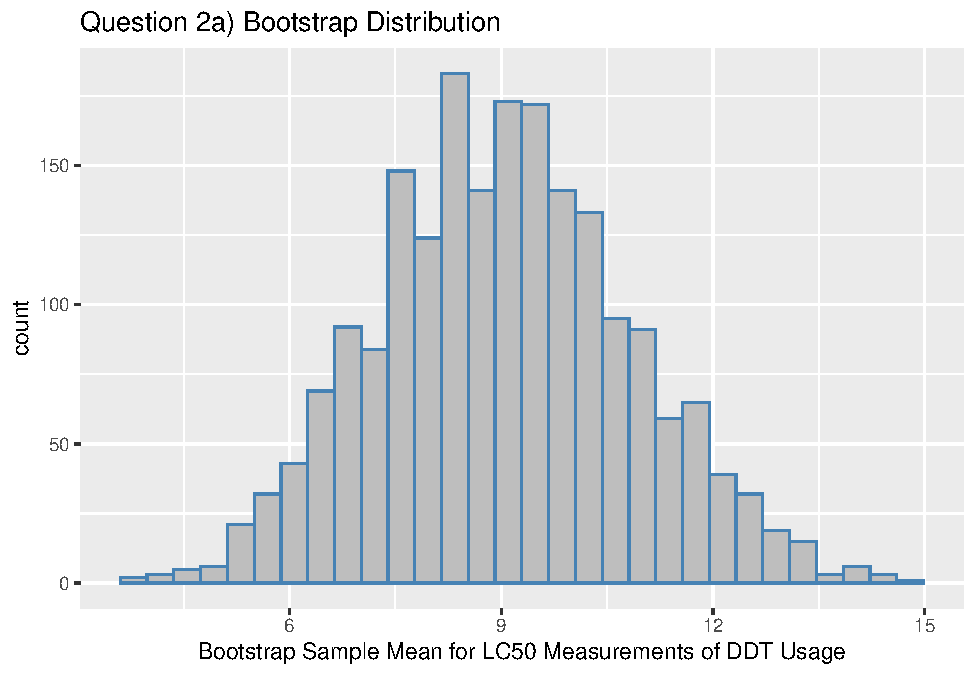
\includegraphics{Assignment1_files/figure-latex/Q2-1.pdf}

\hypertarget{question-2-step-3-4}{%
\subsection{Question 2 Step 3-4}\label{question-2-step-3-4}}

Yes, this is consistent with my thoughts. There is even chance of each
side face appearing, and the simulation shows an even distribution along
each possible side face. Some dice faces are seen more than other, which
is consistent with random independant events.

Step 4: In 3000 simulations of rolling three dice at once and summing
the dice faces, what is the probability the sum is greater or equal to
14? For example, a (5,6,3) outcome sums to 14 and satisfies the
condition sum≥14

\begin{Shaded}
\begin{Highlighting}[]
\CommentTok{\#Step 4}
\NormalTok{nsims }\OtherTok{=} \DecValTok{3000}
\NormalTok{outcome }\OtherTok{=} \FunctionTok{numeric}\NormalTok{(nsims)}
\NormalTok{GE14 }\OtherTok{=} \FunctionTok{numeric}\NormalTok{(nsims)}
\CommentTok{\#Step 4}
\ControlFlowTok{for}\NormalTok{(i }\ControlFlowTok{in} \DecValTok{1}\SpecialCharTok{:}\NormalTok{nsims)\{ }\CommentTok{\#we are going to perform the body of the loop 3000 times}
\NormalTok{    tosses }\OtherTok{=} \FunctionTok{sample}\NormalTok{(}\DecValTok{1}\SpecialCharTok{:}\DecValTok{6}\NormalTok{, }\DecValTok{3}\NormalTok{, }\AttributeTok{replace =} \ConstantTok{TRUE}\NormalTok{)}\CommentTok{\#Toss 3 dices with faces 1:6}
\NormalTok{    outcome[i] }\OtherTok{=} \FunctionTok{sum}\NormalTok{(tosses) }\CommentTok{\#Sum the rolls}
\NormalTok{    GE14[i] }\OtherTok{=} \ControlFlowTok{if}\NormalTok{(outcome[i] }\SpecialCharTok{\textgreater{}=} \DecValTok{14}\NormalTok{) }\DecValTok{1} \ControlFlowTok{else} \DecValTok{0} \CommentTok{\#adds all sums that are greater or equal to 15 to GE14}
\NormalTok{  \}  }\CommentTok{\#close the for{-}loop}
\NormalTok{simresult }\OtherTok{=} \FunctionTok{data.frame}\NormalTok{(outcome) }\CommentTok{\#creates a data frame of the dice sums.}

\CommentTok{\#Step 4 visualization}
\FunctionTok{ggplot}\NormalTok{(simresult, }\FunctionTok{aes}\NormalTok{(}\AttributeTok{x=}\NormalTok{outcome))}\SpecialCharTok{+}
     \FunctionTok{geom\_histogram}\NormalTok{(}\AttributeTok{binwidth =} \DecValTok{1}\NormalTok{, }\AttributeTok{fill =} \StringTok{\textquotesingle{}steelblue\textquotesingle{}}\NormalTok{, }\AttributeTok{color =} \StringTok{\textquotesingle{}black\textquotesingle{}}\NormalTok{, }\AttributeTok{alpha =}\FloatTok{0.7}\NormalTok{)}\SpecialCharTok{+}
     \FunctionTok{labs}\NormalTok{(}\AttributeTok{title =} \StringTok{"Q2 Part 4 Histogram"}\NormalTok{, }\AttributeTok{x =} \StringTok{"Sum of 3000 Die Tosses"}\NormalTok{, }\AttributeTok{y =} \StringTok{"Frequency"}\NormalTok{)}\SpecialCharTok{+}
     \FunctionTok{theme\_minimal}\NormalTok{()}
\end{Highlighting}
\end{Shaded}

\includegraphics{Assignment1_files/figure-latex/Q2b-1.pdf}

\begin{Shaded}
\begin{Highlighting}[]
\CommentTok{\#Step 4 P(Sum\textgreater{}=14)}
\NormalTok{PSumGE14 }\OtherTok{=} \FunctionTok{sum}\NormalTok{(GE14)}\SpecialCharTok{/}\NormalTok{nsims}
\end{Highlighting}
\end{Shaded}

Answer to P(Sum\textgreater=14) for 3 dice tossed and summed, simulation
ran 3000 times. \textbf{0.1623333}

\hypertarget{question-3}{%
\subsection{Question 3}\label{question-3}}

An abbreviated deck of 20 cards consists of four suits (♡,♢,♠,♣) and the
following denominations (10, Jack, Queen, King, Ace).You pick at random
five cards, or a `hand', without replacement.

a)Compute the probability your hand will consist of a 10, Jack, Queen,
King, and Ace of the same suit. One example of such a hand is:
(10♡,J♡,Q♡,K♡,Ace♡)

b)Compute the probability that you get a three-of-a-kind. For example,
(10♡, 10♢, 10♠, J♣, K♡).

c)Compute probability that one observes two Aces and two ♠'s.

\begin{Shaded}
\begin{Highlighting}[]
\NormalTok{TotalPossibilities }\OtherTok{=} \FunctionTok{choose}\NormalTok{(}\DecValTok{20}\NormalTok{,}\DecValTok{5}\NormalTok{) }\CommentTok{\#choosing 5 cards out of a deck of 20}
\NormalTok{Q3a }\OtherTok{=} \DecValTok{4}\SpecialCharTok{*}\DecValTok{1}\SpecialCharTok{/}\NormalTok{TotalPossibilities }\CommentTok{\#4 is the number of suits and 1 is the number of ways we can draw every card of that suit}

\NormalTok{ThreeOfaKind }\OtherTok{=} \FunctionTok{choose}\NormalTok{(}\DecValTok{5}\NormalTok{,}\DecValTok{1}\NormalTok{)}\SpecialCharTok{*}\FunctionTok{choose}\NormalTok{(}\DecValTok{4}\NormalTok{,}\DecValTok{3}\NormalTok{) }\CommentTok{\#Choose the card number multiplied by choosing 3 suits out of 4}
\NormalTok{RemainingTwoCards }\OtherTok{=} \FunctionTok{choose}\NormalTok{(}\DecValTok{16}\NormalTok{,}\DecValTok{2}\NormalTok{) }\CommentTok{\#Choose last two cards from remaining cards}
\NormalTok{Q3b }\OtherTok{=}\NormalTok{ (RemainingTwoCards}\SpecialCharTok{*}\NormalTok{ThreeOfaKind)}\SpecialCharTok{/}\NormalTok{TotalPossibilities}

\NormalTok{BothAcesAreSpades }\OtherTok{\textless{}{-}} \FunctionTok{choose}\NormalTok{(}\DecValTok{3}\NormalTok{, }\DecValTok{2}\NormalTok{)}\SpecialCharTok{*}\FunctionTok{choose}\NormalTok{(}\DecValTok{4}\NormalTok{, }\DecValTok{2}\NormalTok{)}\SpecialCharTok{*}\FunctionTok{choose}\NormalTok{(}\DecValTok{12}\NormalTok{, }\DecValTok{1}\NormalTok{) }\CommentTok{\#Two Aces that are Spades. }
\CommentTok{\#3 choose 2 ways to choose ace that is not a spade as well.}
\CommentTok{\#4 choose 2 ways to pick two spades that are not an Ace}
\CommentTok{\#12 choose 1 way to pick a card that is not an ace}
\NormalTok{OneAceIsSpade }\OtherTok{\textless{}{-}} \FunctionTok{choose}\NormalTok{(}\DecValTok{1}\NormalTok{, }\DecValTok{1}\NormalTok{)}\SpecialCharTok{*}\FunctionTok{choose}\NormalTok{(}\DecValTok{3}\NormalTok{, }\DecValTok{1}\NormalTok{)}\SpecialCharTok{*}\FunctionTok{choose}\NormalTok{(}\DecValTok{4}\NormalTok{,}\DecValTok{1}\NormalTok{)}\SpecialCharTok{*}\FunctionTok{choose}\NormalTok{(}\DecValTok{12}\NormalTok{, }\DecValTok{1}\NormalTok{)}
\NormalTok{Q3c }\OtherTok{=}\NormalTok{ (OneAceIsSpade}\SpecialCharTok{+}\NormalTok{BothAcesAreSpades)}\SpecialCharTok{/}\NormalTok{TotalPossibilities}
\end{Highlighting}
\end{Shaded}

Answer for Part A: \textbf{\ensuremath{2.5799794\times 10^{-4}}}

Answer for Part B: \textbf{0.1547988}

Answer for Part C: \textbf{0.0232198}

\hypertarget{question-4}{%
\subsection{Question 4}\label{question-4}}

An oil and gas executive needs to fly from Calgary, Alberta (airport
code YYC) to Washington-Dulles (airport code IAD) to attend a meeting
with lobbyists about the building of a certain pipeline. Because there
is no direct flight from YYC to IAD, this traveller has fly from YYC to
a different city, then connect with a flight to IAD. The traveler has
airline options. Airline AA will connect through Dallas, Airline UA will
connect through Chicago, or Airline D which connects through
Minneapolis-St.Paul. Taking into their past experiences with flying with
the three airlines in question, this executive hints that the
probability of flying with Airline AA is 0.15. The probability they will
fly with Airline D is three times more than the probability of flying
with Airline UA. Historical data has shown that 15\% of passengers who
fly with Airline AA miss their connecting flights in Dallas. Similarly,
10\% of Airline D passengers and 30\% of Airline UA passengers miss
their connecting flights.

The executive has called the office of the lobby-group to say they have
missed their connecting flight. Compute the probability that the
executive called from Chicago (or is flying Airline UA).

\begin{Shaded}
\begin{Highlighting}[]
\NormalTok{AirlineAAProb }\OtherTok{=} \FloatTok{0.15}
\NormalTok{AirlineUAProb }\OtherTok{=} \FloatTok{0.2125} \CommentTok{\#Algebra, 1 = 0.15+3x+x solve for x}
\NormalTok{AirlineDProb }\OtherTok{=} \DecValTok{3}\SpecialCharTok{*}\NormalTok{AirlineUAProb}

\NormalTok{AirlineAAMiss }\OtherTok{=} \FloatTok{0.15}
\NormalTok{AirlineUAMiss }\OtherTok{=} \FloatTok{0.30}
\NormalTok{AirlineDMiss }\OtherTok{=} \FloatTok{0.1}

\NormalTok{ChancesToMiss }\OtherTok{=}\NormalTok{ (AirlineAAMiss}\SpecialCharTok{*}\NormalTok{AirlineAAProb)}\SpecialCharTok{+}\NormalTok{(AirlineDMiss}\SpecialCharTok{*}\NormalTok{AirlineDProb)}\SpecialCharTok{+}\NormalTok{(AirlineUAMiss}\SpecialCharTok{*}\NormalTok{AirlineUAProb) }\CommentTok{\#All situations where the flight is missed}
\NormalTok{Q4 }\OtherTok{=}\NormalTok{ AirlineUAProb}\SpecialCharTok{*}\NormalTok{AirlineUAMiss}\SpecialCharTok{/}\NormalTok{ChancesToMiss }\CommentTok{\#UA is missed divided by chances to miss. }
\end{Highlighting}
\end{Shaded}

Answer: \textbf{0.425}

\hypertarget{question-5}{%
\subsection{Question 5}\label{question-5}}

A random variable X has the following probability distribution function
P(X=x)=2/3\^{}(x+1) x=0,1,2,⋯

a)Using R Studio, create a display that shows the probability
distribution of this particular random variable X. Refer to the various
code provided for examples appearing in both Probability Module 4 and
Review Exercise 5 from Thursday, September 8th. For values of x, use
xvalues = 0:15.

\begin{enumerate}
\def\labelenumi{\alph{enumi})}
\setcounter{enumi}{1}
\tightlist
\item
  How likely is it to observe values beyond 4? Compute
  P(X\textgreater4). c)Compute the mean or expected value of X, E(X)or
  μX. (Hint: In computing E(X), change the upper limit on xvalues from
  15 to 100\ldots) d)Compute the standard deviation of X, SD(X) or σX.
  (use the same values of x as you did in part (c)) e)Consider the
  interval (μX−σX,μX+σX). Compute P(μX−σX \textless X\textless{} μX+σX).
\end{enumerate}

\begin{Shaded}
\begin{Highlighting}[]
\NormalTok{PX }\OtherTok{=} \ControlFlowTok{function}\NormalTok{(x) \{ }\CommentTok{\#Function described in the question}
  \DecValTok{2}\SpecialCharTok{/}\NormalTok{(}\DecValTok{3}\SpecialCharTok{\^{}}\NormalTok{(x }\SpecialCharTok{+} \DecValTok{1}\NormalTok{))}
\NormalTok{\}}
\NormalTok{x }\OtherTok{=} \DecValTok{0}\SpecialCharTok{:}\DecValTok{15}
\NormalTok{xProbabilites }\OtherTok{=} \FunctionTok{PX}\NormalTok{(x)}
\NormalTok{Q5b }\OtherTok{=} \FunctionTok{sum}\NormalTok{(xProbabilites[x}\SpecialCharTok{\textgreater{}}\DecValTok{4}\NormalTok{])}

\NormalTok{EVpx }\OtherTok{=} \ControlFlowTok{function}\NormalTok{(x) \{ }\CommentTok{\#Function times x to find expected value}
\NormalTok{  x}\SpecialCharTok{*}\NormalTok{(}\DecValTok{2}\SpecialCharTok{/}\NormalTok{(}\DecValTok{3}\SpecialCharTok{\^{}}\NormalTok{(x }\SpecialCharTok{+} \DecValTok{1}\NormalTok{)))}
\NormalTok{\}}
\NormalTok{x }\OtherTok{=} \DecValTok{0}\SpecialCharTok{:}\DecValTok{100}
\NormalTok{Q5c }\OtherTok{=} \FunctionTok{sum}\NormalTok{(}\FunctionTok{EVpx}\NormalTok{(x))}

\NormalTok{m2 }\OtherTok{=} \ControlFlowTok{function}\NormalTok{(x) \{ }\CommentTok{\#Function times x squared to find variance}
\NormalTok{  (x}\SpecialCharTok{\^{}}\DecValTok{2}\NormalTok{)}\SpecialCharTok{*}\NormalTok{(}\DecValTok{2}\SpecialCharTok{/}\NormalTok{(}\DecValTok{3}\SpecialCharTok{\^{}}\NormalTok{(x }\SpecialCharTok{+} \DecValTok{1}\NormalTok{)))}
\NormalTok{\}}
\NormalTok{variance }\OtherTok{=} \FunctionTok{sum}\NormalTok{(}\FunctionTok{m2}\NormalTok{(x))}
\NormalTok{Q5d }\OtherTok{=} \FunctionTok{sqrt}\NormalTok{(variance}\SpecialCharTok{{-}}\NormalTok{Q5c}\SpecialCharTok{\^{}}\DecValTok{2}\NormalTok{)}

\NormalTok{x }\OtherTok{=} \DecValTok{0}\SpecialCharTok{:}\DecValTok{100}
\NormalTok{lower\_bound }\OtherTok{=}\NormalTok{ Q5c}\SpecialCharTok{{-}}\NormalTok{Q5d}
\NormalTok{upper\_bound }\OtherTok{=}\NormalTok{ Q5c}\SpecialCharTok{+}\NormalTok{Q5d}
\NormalTok{Q5e }\OtherTok{=}  \FunctionTok{sum}\NormalTok{(xProbabilites[(x }\SpecialCharTok{\textgreater{}}\NormalTok{ Q5c }\SpecialCharTok{{-}}\NormalTok{ Q5d) }\SpecialCharTok{\&}\NormalTok{ (x }\SpecialCharTok{\textless{}}\NormalTok{ Q5c }\SpecialCharTok{+}\NormalTok{ Q5d)])}
\end{Highlighting}
\end{Shaded}

Answer for Part A:

\begin{Shaded}
\begin{Highlighting}[]
\NormalTok{x }\OtherTok{=} \DecValTok{0}\SpecialCharTok{:}\DecValTok{15}
\FunctionTok{plot}\NormalTok{(x, xProbabilites, }\AttributeTok{xlab=}\StringTok{"Values of X"}\NormalTok{,}\AttributeTok{ylab =} \StringTok{"Density of f(x)"}\NormalTok{, }\AttributeTok{main =} \StringTok{"Distribution of X"}\NormalTok{, }\AttributeTok{col =} \StringTok{\textquotesingle{}red\textquotesingle{}}\NormalTok{)}
\end{Highlighting}
\end{Shaded}

\includegraphics{Assignment1_files/figure-latex/Q5a-1.pdf}

Answer for Part B: \textbf{0.0041152}

Answer for Part C: \textbf{0.5}

Answer for Part D: \textbf{0.8660254}

Answer for Part E: \textbf{0.8888889}

\hypertarget{question-6}{%
\subsection{Question 6}\label{question-6}}

\begin{enumerate}
\def\labelenumi{\alph{enumi})}
\tightlist
\item
  Create a bar graph that demonstrates the distribution of race within
  each level of education. What can you infer from this bar graph?
\item
  Create a data visualization that can be used to demonstrate if there
  is a relationship between one's marital status (Marital) and their
  education level. c)Create a data visualization that can be used to
  demonstrate if there is a relationship between one's Gender and their
  Politics.
\end{enumerate}

\begin{Shaded}
\begin{Highlighting}[]
\NormalTok{gss }\OtherTok{=} \FunctionTok{read.csv}\NormalTok{(}\StringTok{"https://raw.githubusercontent.com/Statman44/Data602/main/GSS2002.csv"}\NormalTok{)}

\CommentTok{\#Part A}
\FunctionTok{ggplot}\NormalTok{(gss, }\FunctionTok{aes}\NormalTok{(}\AttributeTok{x=}\NormalTok{Education, }\AttributeTok{fill =}\NormalTok{ Race))}\SpecialCharTok{+}
  \FunctionTok{geom\_bar}\NormalTok{(}\AttributeTok{position=}\StringTok{"dodge"}\NormalTok{, }\AttributeTok{na.rm=}\ConstantTok{TRUE}\NormalTok{)}\SpecialCharTok{+}
  \FunctionTok{labs}\NormalTok{(}\AttributeTok{title=}\StringTok{"Question 6 Part A"}\NormalTok{, }\AttributeTok{x=}\StringTok{"Education Level"}\NormalTok{, }\AttributeTok{y=}\StringTok{"Count"}\NormalTok{)}\SpecialCharTok{+}
  \FunctionTok{theme\_minimal}\NormalTok{()}
\end{Highlighting}
\end{Shaded}

\includegraphics{Assignment1_files/figure-latex/Q6-1.pdf}

\begin{Shaded}
\begin{Highlighting}[]
\CommentTok{\#Part B}
\FunctionTok{ggplot}\NormalTok{(gss, }\FunctionTok{aes}\NormalTok{(}\AttributeTok{x=}\NormalTok{Marital, }\AttributeTok{fill =}\NormalTok{ Education))}\SpecialCharTok{+}
  \FunctionTok{geom\_bar}\NormalTok{(}\AttributeTok{position=}\StringTok{"dodge"}\NormalTok{, }\AttributeTok{na.rm=}\ConstantTok{TRUE}\NormalTok{)}\SpecialCharTok{+}
  \FunctionTok{labs}\NormalTok{(}\AttributeTok{title=}\StringTok{"Question 6 Part B"}\NormalTok{, }\AttributeTok{x=}\StringTok{"Marital Status"}\NormalTok{, }\AttributeTok{y=}\StringTok{"Count"}\NormalTok{)}\SpecialCharTok{+}
  \FunctionTok{theme\_minimal}\NormalTok{()}
\end{Highlighting}
\end{Shaded}

\includegraphics{Assignment1_files/figure-latex/Q6-2.pdf}

\begin{Shaded}
\begin{Highlighting}[]
\CommentTok{\#Part C}
\FunctionTok{ggplot}\NormalTok{(gss, }\FunctionTok{aes}\NormalTok{(}\AttributeTok{x=}\NormalTok{Gender, }\AttributeTok{fill =}\NormalTok{ Politics))}\SpecialCharTok{+}
  \FunctionTok{geom\_bar}\NormalTok{(}\AttributeTok{position=}\StringTok{"dodge"}\NormalTok{, }\AttributeTok{na.rm=}\ConstantTok{TRUE}\NormalTok{)}\SpecialCharTok{+}
  \FunctionTok{labs}\NormalTok{(}\AttributeTok{title=}\StringTok{"Question 6 Part C"}\NormalTok{, }\AttributeTok{x=}\StringTok{"Gender"}\NormalTok{, }\AttributeTok{y=}\StringTok{"Count"}\NormalTok{)}\SpecialCharTok{+}
  \FunctionTok{theme\_minimal}\NormalTok{()}
\end{Highlighting}
\end{Shaded}

\includegraphics{Assignment1_files/figure-latex/Q6-3.pdf}

Answer for Part A: In every level of education listed, white people have
higher counts than other races. They also have higher counts of leaving
High School than other races. I infer this is because the raw counts of
white people are higher than other races.

\hypertarget{question-7}{%
\subsection{Question 7}\label{question-7}}

\begin{enumerate}
\def\labelenumi{\arabic{enumi}.}
\setcounter{enumi}{6}
\tightlist
\item
  Refer to the Default data set in the ISLR package. This data set
  consists of 10000 cases. There are four different variables in this
  data set. ``default'' is a categorical variable that indicates if a
  person has defaulted on their credit card debt (Yes) or has not (No);
  the variable ``student'' flags a respondent as a student (Yes) or not
  (No); the third variable is the person's credit card balancing they
  are carrying, and the last variable ``income'' is the person's annual
  income.
\end{enumerate}

a)Create a scatterplot that demonstrates the relationship between a
person's income and their monthly balance they carry on their credit
cards. Place the ``income'' variable as the y-axis and the ``balance''
variable as the x-axis. Within this visualization, differentiate between
those who are students and those who are not.

b)Create side-by-side boxplots that will compare the distributions of
balance owing between students and non-students.

c)Compute the means, medians, standard deviations, x5, x95 (the 5th and
95th percentiles, respectively) for the data you visually summarized in
part (b).

\begin{Shaded}
\begin{Highlighting}[]
\FunctionTok{library}\NormalTok{(ISLR)}
\FunctionTok{head}\NormalTok{(Default, }\DecValTok{4}\NormalTok{)}
\end{Highlighting}
\end{Shaded}

\begin{verbatim}
##   default student   balance   income
## 1      No      No  729.5265 44361.63
## 2      No     Yes  817.1804 12106.13
## 3      No      No 1073.5492 31767.14
## 4      No      No  529.2506 35704.49
\end{verbatim}

\begin{Shaded}
\begin{Highlighting}[]
\CommentTok{\#Part a}
\FunctionTok{ggplot}\NormalTok{(Default, }\FunctionTok{aes}\NormalTok{(}\AttributeTok{x =}\NormalTok{balance, }\AttributeTok{y =}\NormalTok{ income, }\AttributeTok{color =}\NormalTok{ student))}\SpecialCharTok{+}
  \FunctionTok{geom\_point}\NormalTok{(}\AttributeTok{alpha =} \FloatTok{0.7}\NormalTok{)}\SpecialCharTok{+}
  \FunctionTok{labs}\NormalTok{(}\AttributeTok{title =} \StringTok{"Question 7 Scatter Plot"}\NormalTok{, }\AttributeTok{x =} \StringTok{"Balance"}\NormalTok{, }\AttributeTok{y =}\StringTok{"Income"}\NormalTok{)}\SpecialCharTok{+}
  \FunctionTok{theme\_minimal}\NormalTok{()}
\end{Highlighting}
\end{Shaded}

\includegraphics{Assignment1_files/figure-latex/Q7-1.pdf}

\begin{Shaded}
\begin{Highlighting}[]
\CommentTok{\#Part b}
\FunctionTok{ggplot}\NormalTok{(Default, }\FunctionTok{aes}\NormalTok{(}\AttributeTok{x =}\NormalTok{student, }\AttributeTok{y =}\NormalTok{ balance, }\AttributeTok{fill =}\NormalTok{ student))}\SpecialCharTok{+}
  \FunctionTok{geom\_boxplot}\NormalTok{()}\SpecialCharTok{+}
  \FunctionTok{labs}\NormalTok{(}\AttributeTok{title =} \StringTok{"Question 7 Scatter Plot"}\NormalTok{, }\AttributeTok{x =} \StringTok{"Balance"}\NormalTok{, }\AttributeTok{y =}\StringTok{"Income"}\NormalTok{, }\AttributeTok{fill =} \StringTok{"Student"}\NormalTok{)}\SpecialCharTok{+}
  \FunctionTok{theme\_minimal}\NormalTok{()}
\end{Highlighting}
\end{Shaded}

\includegraphics{Assignment1_files/figure-latex/Q7-2.pdf}

\begin{Shaded}
\begin{Highlighting}[]
\CommentTok{\#Part c}
\CommentTok{\#Student Stats}
\NormalTok{calc\_stats }\OtherTok{\textless{}{-}} \ControlFlowTok{function}\NormalTok{(data) \{}
\NormalTok{  mean\_val }\OtherTok{\textless{}{-}} \FunctionTok{mean}\NormalTok{(data, }\AttributeTok{na.rm =} \ConstantTok{TRUE}\NormalTok{)}
\NormalTok{  median\_val }\OtherTok{\textless{}{-}} \FunctionTok{median}\NormalTok{(data, }\AttributeTok{na.rm =} \ConstantTok{TRUE}\NormalTok{)}
\NormalTok{  sd\_val }\OtherTok{\textless{}{-}} \FunctionTok{sd}\NormalTok{(data, }\AttributeTok{na.rm =} \ConstantTok{TRUE}\NormalTok{)}
\NormalTok{  x5\_val }\OtherTok{\textless{}{-}} \FunctionTok{quantile}\NormalTok{(data, }\FloatTok{0.05}\NormalTok{, }\AttributeTok{na.rm =} \ConstantTok{TRUE}\NormalTok{)}
\NormalTok{  x95\_val }\OtherTok{\textless{}{-}} \FunctionTok{quantile}\NormalTok{(data, }\FloatTok{0.95}\NormalTok{, }\AttributeTok{na.rm =} \ConstantTok{TRUE}\NormalTok{)}
  
  \FunctionTok{return}\NormalTok{(}\FunctionTok{c}\NormalTok{(}\AttributeTok{Mean =}\NormalTok{ mean\_val, }\AttributeTok{Median =}\NormalTok{ median\_val, }\AttributeTok{StandardDeviation =}\NormalTok{ sd\_val, }\AttributeTok{x5 =}\NormalTok{ x5\_val, }\AttributeTok{x95 =}\NormalTok{ x95\_val))}
\NormalTok{\}}

\NormalTok{StudentStats }\OtherTok{\textless{}{-}} \FunctionTok{calc\_stats}\NormalTok{(Default}\SpecialCharTok{$}\NormalTok{balance[Default}\SpecialCharTok{$}\NormalTok{student }\SpecialCharTok{==} \StringTok{"Yes"}\NormalTok{])}
\NormalTok{NonStudentStats }\OtherTok{\textless{}{-}} \FunctionTok{calc\_stats}\NormalTok{(Default}\SpecialCharTok{$}\NormalTok{balance[Default}\SpecialCharTok{$}\NormalTok{student }\SpecialCharTok{==} \StringTok{"No"}\NormalTok{])}
\NormalTok{stats\_df }\OtherTok{\textless{}{-}} \FunctionTok{data.frame}\NormalTok{(}\FunctionTok{rbind}\NormalTok{(}\AttributeTok{Student =}\NormalTok{ StudentStats, }\AttributeTok{NonStudent =}\NormalTok{ NonStudentStats))}

\CommentTok{\#Table \textless{}{-} kable(stats\_df, format = "html") \%\textgreater{}\% kable\_styling()}
\end{Highlighting}
\end{Shaded}

Answer for Part C: r Table

\end{document}
